\documentclass[a4paper,11pt]{article}
%\documentclass[a4paper,11pt]{article}

\usepackage[latin1]{inputenc}
%\usepackage{epsfig}
%\usepackage{color}
\usepackage{mathrsfs}
\usepackage{amsmath,amssymb}
%\usepackage{ifthen}
%\usepackage[normalem]{ulem}
\usepackage{url}
\usepackage{graphicx}
%\usepackage{xspace}

\usepackage{natbib}

% \usepackage{vmargin}
% \setpapersize[portrait]{A4}
% \setmarginsrb{35mm}{30mm}{35mm}{25mm}% left, top, right, bottom
% {0pt}{0mm}% head heigth / separation
% {12pt}{15mm}% bottom height / separation


%%%%%%%%%%%%%%%%%%%%%%%%%%%%%%%%%%%%%%%%%%%%%%%%%%%%%%%%%%%%%%%%%%%%%%
%% title, authors, running heads

\title{The \texttt{zipfR} package for lexical statistics:\\
  A tutorial introduction}

\date{23 August 2006\\
  \texttt{zipfR} version 0.6-0}

\author{Marco Baroni \and Stefan Evert}


%%%%%%%%%%%%%%%%%%%%%%%%%%%%%%%%%%%%%%%%%%%%%%%%%%%%%%%%%%%%%%%%%%%%%%
%% some macro definitions

%% ... \TODO{something missing here} ...
\newcommand{\TODO}[1]{{$\bigl[\![$\marginpar{\textbf{\small TODO}}\textit{#1}$]\!\bigr]$}}
%% ... \CITE{missing citation} ...
\newcommand{\CITE}[1]{{$\bigl[$\marginpar{\textbf{\small REF}}#1$\bigr]$}}

%%%%%%%%%%%%%%%%%%%%%%%%%%%%%%%%%%%%%%%%%%%%%%%%%%%%%%%%%%%%%%%%%%%%%%
%% the main text

\begin{document}

\maketitle

%%%%%%%%%%%%%%%%%%%%%%%%%%%%%%%%%%%%%%%%%%%%%%%%%%%%%%%%%%%%%%%%%%%%%%
%%  1  Motivation

\section{Introduction}

This document provides a tutorial introduction to the zipfR package
\citep{Evert:Baroni:2006b} for Large-Number-of-Rare-Events (LNRE)
modeling of lexical distributions \citep{Baayen:2001}. We assume that
R is installed on your computer and that you have basic familiarity
with it. If this is not the case, please start by visiting the R page
at \url{http://www.r-project.org/}. The page provides links to
download sites, documentation and introductory material. For an
elementary book-length introduction to doing statistics with R, see
\citet{Dalgaard:2002}.

\section{Installing and loading zipfR}

The zipfR package is available on CRAN, the central R repository. If
you are using the R graphical user interface under Mac OS X or
Windows, installing zipfR should be as easy as selecting Package
Installer from the Packages \& Data menu, getting a list of the CRAN
binaries, looking for zipfR, selecting it and clicking on the Install
Selected button (there might be small differences between operating
systems and among R versions, but the Package Installer is very user
friendly, and the steps to take should always be fairly obvious).

If you are using the command line version on Linux or other Unix
platform, see the documentation for \texttt{install.packages} and
related functions:

\begin{verbatim}
> ?install.packages
\end{verbatim}

Please take a look at the R documentation for detailed instructions on
how to install packages stored on CRAN (such instructions will also
apply to zipfR).

Whenever you intend to access zipfR functionalities during a R
session, you have to load it. If you are using the graphical user
interface, you can select Package Manager from the Packages \& Data
menu (or similar) and load the package through the graphical
options. Both on the command line and on the GUI, you can also load
zipfR as follows:

\begin{verbatim}
> library(zipfR)
\end{verbatim}

Once zipfR has been loaded, you can browse its documentation with the
command:

\begin{verbatim}
> ?zipfR
\end{verbatim}


\section{Case study 1: Estimating vocabulary size of a productive
  process}

We illustrate the basic functionalities of the package by considering
a classic problem in quantitative linguistics, i.e., that of
estimating the number of distinct \emph{types} that belong to a
certain category, given a sample of \emph{tokens} from the relevant
category. Our example data come from the Italian word formation
process of \emph{ri-} prefixation (comparable, although not identical,
to English \emph{re-} prefixation). The data were extracted from a 380
million token corpus of newspaper Italian \citep{Baroni:etal:2004},
and they consist of all verbal lemmas beginning with the prefix
\emph{ri-} in the corpus (extracted with a mixture of automated
methods and manual checking).

Morphology has been a traditional field of application of lexical
statistics (see, e.g., \citealp{Baayen:1992}), although the general
problem of computing the number of types (vocabulary size) in a
population given a sample from the population is also relevant to many
other language-related fields, from stylometry (estimating the
vocabulary size of different authors) to syntax (measuring the size
and productivity of word classes and constructions) to language
acquisition (measuring lexical richness of children or language
learners).

We will use the symbol $V$ for vocabulary size (number of types), $N$
for sample size (number of tokens) and $V_{m}$ ($m$ an integer value)
for the number of types that have frequency $m$. In particular, $V_1$
is the number of \emph{hapax legomena}, i.e., the number of types that
occur only once in the corpus.

\subsection{Frequency spectra}

If you have an open R session and you loaded zipfR, you can read in
the \emph{ri-} frequency data with the following command:

\begin{verbatim}
> data(ItaRi.spc)
\end{verbatim}

The object \texttt{ItaRi.spc} is a \textbf{frequency spectrum}, the
most important data structure in zipfR. A frequency spectrum
summarizes a frequency distribution in terms of number of types
($V_{m}$) per frequency class ($m$), i.e., it reports how many
distinct types occur once, how many types occur twice, and so on. For
example, the first few rows of the \texttt{ItaRi.spc} spectrum (which
we can inspect by typing the object name) are:

\begin{verbatim}
> ItaRi.spc
    m  Vm
1   1 346
2   2 105
3   3  74
4   4  43
5   5  39
6   6  25
7   7  27
8   8  15
9   9  17
10 10   9
	...

       N    V
 1399898 1098
\end{verbatim}

% \begin{quote}
%   \begin{tabular}{l|r}
%     $m$ & $V_{m}$\\
%     \hline
%     1 & 346\\
%     2 & 105\\
%     3 & 74\\
%     4 & 43\\
%     5 & 39\\
%   \end{tabular}
% \end{quote}
Thus, we see that in our corpus there are 412 \emph{ri-} verbs that
occur once, 119 \emph{ri-} verbs that occur twice, etc.

General information about the spc data structure can be found in the
help entry for \texttt{spc}. For information on reading your own
frequency spectrum into R from a tab-delimited text file (and saving a
spectrum object to an output text file), take a look at the
documentation for the \texttt{read.spc} and \texttt{write.spc}
functions. You can also import a type frequency list (a list of
frequencies of the linguistic entities of interest) and generate a
spectrum file from it: see documentation for the \texttt{read.tfl} and
\texttt{tfl2spc} functions (while we do not discuss it further here,
the zipfR \textbf{type frequency list} object is of fundamental
practical importance, given that input data will often be in the form
of frequency lists; see the \texttt{tfl} documentation entry).

The zipfR package provides various utility functions to explore the
frequency distribution encoded in a spectrum object. First,
\texttt{summary} applied to a spectrum data structure returns a useful
sketch of the spectrum ($N$, $V$, the type frequencies of the first
few classes of the spectrum):

\begin{verbatim}
> summary(ItaRi.spc)
zipfR object for frequency spectrum
Sample size:     N  = 1399898 
Vocabulary size: V  = 1098 
Class sizes:     Vm = 346 105 74 43 39 25 27 15 ...
\end{verbatim}

The function \texttt{summary} can be applied to most zipfR data
structures, to obtain basic information about the structure
contents. The function \texttt{N} returns the sample size $N$,
\texttt{V} returns the vocabulary size $V$:

\begin{verbatim}
> N(ItaRi.spc)
[1] 1399898
> V(ItaRi.spc)
[1] 1098
\end{verbatim}

You can use \texttt{N} and \texttt{V} with any zipfR object for which
$N$ and $V$ constitute relevant information (although you might get
different types of information: see the documentation for these
functions). The function \texttt{Vm} returns the number of types with
frequency $m$; if the argument specifying $m$ is a vector, it returns
a vector containing the number of types for the specified range of
spectrum elements:

\begin{verbatim}
> Vm(ItaRi.spc,1)
[1] 346
> Vm(ItaRi.spc,1:5)
[1] 346 105  74  43  39
\end{verbatim}

You can use \texttt{Vm} and \texttt{N} to compute the famous
$\mathscr{P}$ measure of productivity proposed by Harald Baayen (see,
e.g., \citealp{Baayen:1992}). $\mathscr{P}$ is obtained by dividing
the number of hapax legomena by the overall sample size:

\begin{verbatim}
> Vm(ItaRi.spc,1) / N(ItaRi.spc)
[1] 0.0002471609
\end{verbatim}

It is informative to obtain a plot of a spectrum file, with $m$ on the
$x$ axis and $V_{m}$ on the $y$ axis. Here are three ways to do this:

\begin{verbatim}
> plot(ItaRi.spc)
> plot(ItaRi.spc, log="x")
> plot.default(ItaRi.spc, main="Frequency Spectrum")
\end{verbatim}

The resulting plots:

\begin{center}
  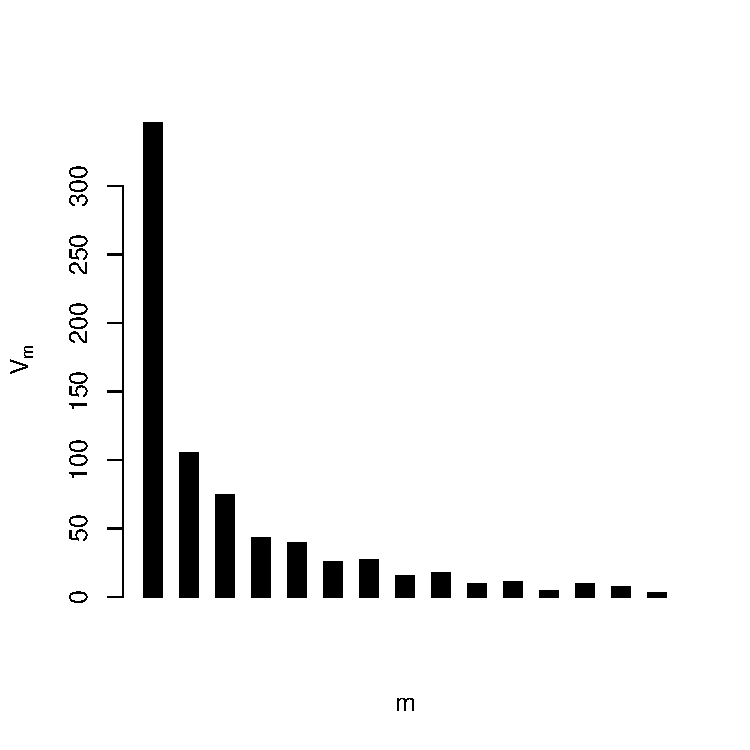
\includegraphics[width=6cm]{img/ri-spc-linear}
  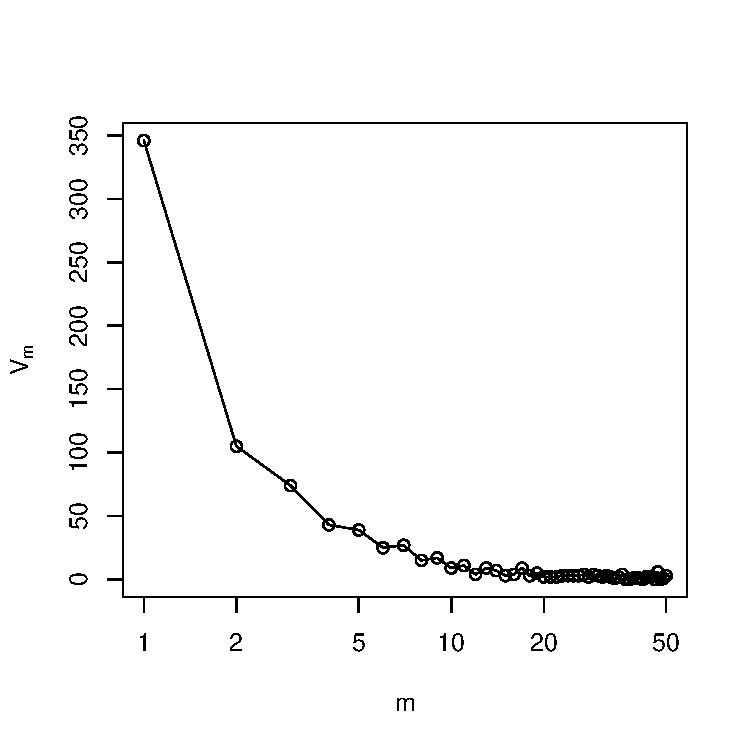
\includegraphics[width=6cm]{img/ri-spc-log-x}
  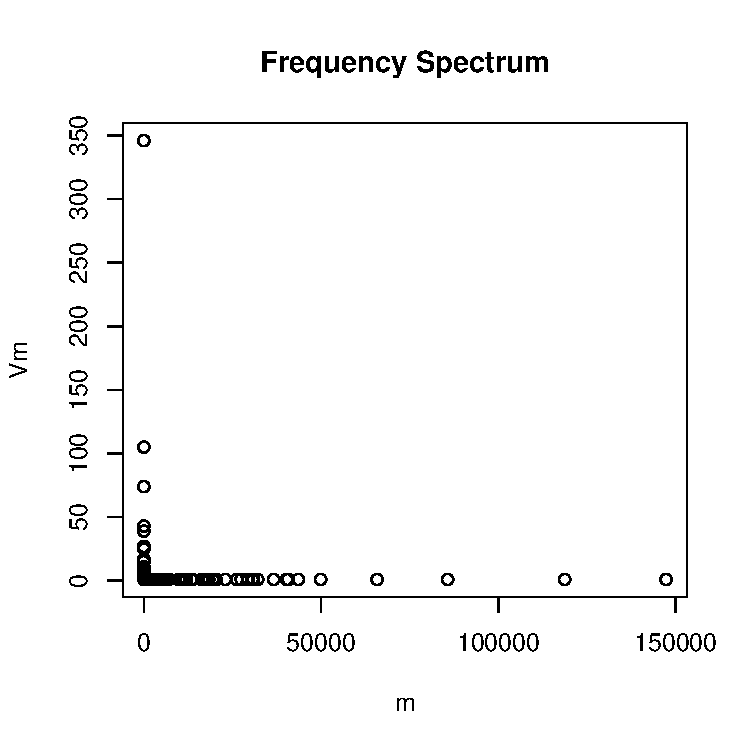
\includegraphics[width=6cm]{img/ri-spc-default}
\end{center}

As the first figure shows, applying the function \texttt{plot} to a zipfR
spectrum with no other arguments produces a histogram of the first 15
frequency classes in the spectrum. If the argument \texttt{log="x"} is passed,
we obtain by default a plot of the first 50 spectrum elements with the $x$
(i.e., $m$) axis on a logarithmic scale, as illustrated in the second
figure. The last figure shows why \texttt{plot} applied to a spectrum does not
generate a plot of the full range of frequency classes. A spectrum is often
characterized by very high values corresponding to the lowest frequency
classes, and a very long tail of frequency classes with only one member (i.e.,
just one word with frequency 100, just one word with frequency 103, etc.)
Thus, a full spectrum plot on non-logarithmic scale will have the rather
uninformative L-shaped profile we see in the third figure (generated with the
standard scatterplot function \texttt{plot.default}).

The zipfR functions try to provide reasonable default values for all
parameters that are not specified in a function call, making it very
easy to obtain basic plots of the desired data structures. The
defaults can of course be overridden. For example, you can pass a
different title through the \texttt{main} argument, or use
\texttt{xlab} and \texttt{ylab} to change the axis labels. For more
information on the plotting parameters, look at the help for
\texttt{plot.spc}. In case you need even finer control over the
parameters, a zipfR spectrum (like most other zipfR data structures)
is also typed as a regular R dataframe, which means that you can
access its contents with standard R syntax (\texttt{ItaRi.spc\$m,
  ItaRi.spc\$Vm}). Keep in mind, however, that the results of directly
accessing the data structure might not be what you expect (e.g.,
\texttt{ItaRi.spc\$Vm[50]} does not necessarily return the value of
$V_{50}$, but the value of the 50th \emph{non-zero} frequency class!)

Once you have generated a plot, you can export it in pdf or other
formats using standard R functionalities (e.g., if you are using the
Mac OS X GUI, through the \texttt{pdf} device or by selecting Save
As\ldots{} from the File menu).


\subsection{Vocabulary growth curves}

Frequency spectrum plots provide valuable information about the nature
of a process: if, as is the case with \emph{ri-}, a process is
characterized by a high proportion of hapax legomena and other low
frequency classes, this indicates that the process is productive,
i.e., the chances that if we were to sample more tokens of the same
category we would encounter new types are high.

In order to develop an intuition about how rapidly vocabulary size is
growing, another type of data structure (and associated plot) is more
informative, i.e., the \emph{vocabulary growth curve}. A vocabulary
growth curve reports vocabulary size (number of types, $V$) as a
function of sample size (number of tokens, $N$). The data necessary to
plot an \emph{empirical} vocabulary growth curve (we discuss
\emph{interpolated} and \emph{extrapolated} vgcs below) cannot be
derived from a single frequency spectrum, since the spectrum is only
providing us with information about a single sample size, and we do
not know how ``we got there''. Consider, for example, the two
``corpora'' \texttt{a b a b a b a b} and \texttt{a a a a b b b b}:
they have the same frequency spectrum, but different vocabulary growth
curves.

Vocabulary growth data can be imported into the \textbf{vocabulary
  growth curve} (\emph{vgc}) data structure, that will contain $V$
values for increasing $N$s. Moreover, the zipfR vgc data structure can
have optional columns from $V_1$ to $V_9$, reporting the number of
types in the corresponding frequency classes at the specified $N$s
(how many distinct types have frequency 1, how many types have
frequency 2, etc.)  The most interesting frequency class is typically
that of hapax legomena; thus, often we find ourselves working with
vgcs that contain the fields $N$, $V$ and $V_1$. As a case in point,
you can load the empirical vgc for the \emph{ri-} data as follows:

\begin{verbatim}
> data(ItaRi.emp.vgc)
\end{verbatim}

The first few rows of this structure (inspected with the handy
function \texttt{head}) are:

\begin{verbatim}
> head(ItaRi.emp.vgc)
     N   V V1
1 1000 140 62
2 2000 178 58
3 3000 201 60
4 4000 211 53
5 5000 224 61
6 6000 235 59
\end{verbatim}

% \begin{quote}
%   \begin{tabular}{l|r|r}
%     $N$ & $V$ & $V_1$\\
%     \hline
%     1,000 &140 &62\\
%     2,000 &178 &58\\
%     3,000 &201 &60\\
%     4,000 &211 &53\\
%     5,000 &224 &61\\
%   \end{tabular}
% \end{quote}
This indicates that, after the first 1,000 \emph{ri-} tokens in the
target corpus, we saw 140 distinct \emph{ri-} types, 62 of them having
occurred only once at that point; after the first 2,000 tokens, we saw
178 distinct types, 58 of them being hapax legomena at that point; and
so on. For instructions on how to import your vgcs from tab-delimited
text files and more information about this data structure, browse the
documentation for \texttt{read.vgc} and \texttt{vgc}.

If you simply print the \texttt{vgc} object, a random selection of 25 rows
will be shown to give you a general overview of the vocabulary development
(the output is truncated in the example below).  From the corresponding
summary, you can see how many samples are included in the vocabulary growth
curve:

\begin{verbatim}
> ItaRi.emp.vgc
           N    V  V1
71     71000  441 123
125   125000  516 158
...
1251 1251000 1045 317
1334 1334000 1075 334
	(random subset of 25 entries shown)

> summary(ItaRi.emp.vgc)
zipfR object for vocabulary growth curve
1400 samples for N = 1000 ... 1399898 
Spectrum elements included up to m = 1 
\end{verbatim}

A vocabulary growth plot (with $V$ and $V_1$ curves) can be created
with the following command:

\begin{verbatim}
> plot(ItaRi.emp.vgc, add.m=1)
\end{verbatim}

By specifying \texttt{add.m=1}, we ask for $V_1$ to be plotted as well
(it appears as a thinner line below $V$). The command produces the
following plot:

\begin{center}
  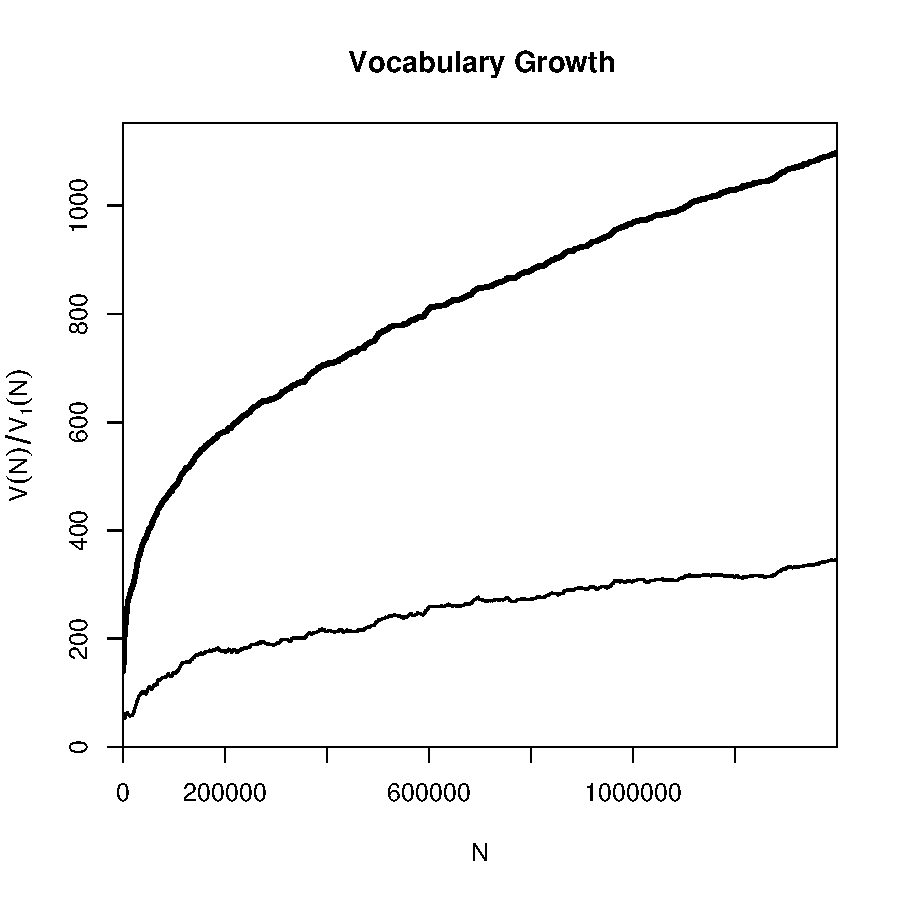
\includegraphics[width=6cm]{img/ri-vgc-v-v1}
\end{center}

More information about plotting vgcs is available on the
\texttt{plot.vgc} help page.


\subsection{Interpolation}
\label{interpolation}

An \emph{empirical} growth curve such as the one we just plotted is
typically not very smooth, as it reflects all the quirks due to the
non-random distribution of words and texts in a corpus. A smoother
curve can be obtained with the technique of \emph{binomial
  interpolation} \citep[ch.~2]{Baayen:2001}. Given a frequency
spectrum, binomial interpolation produces the \emph{expected values}
of vocabulary size (and number of types in specific frequency classes
-- e.g., number of hapax legomena) for arbitrary sample sizes (smaller
or equal to the sample size at which the spectrum has been computed).
These expected values can be thought of as the average of vocabulary
size (or other measures) computed over a large number of
randomizations of the order of tokens in the corpus. Notice that
expected values, unlike observed counts, are not necessarily integers.

We can obtain an interpolated vocabulary growth curve even when we only have a
spectrum or frequency list. For example, we can compute an interpolated growth
curve from the \emph{ri-} spectrum as follows:%
\footnote{Note that the \texttt{+} sign at the start of the second line
  indicates that the full command does not fit into a single line and has
  spilled over to the following line (\texttt{+} is the prompt that R uses
  when you have entered an incomplete command).  Simply type the entire
  command (with all continuation lines) on a single line when you run these
  examples.}

\begin{verbatim}
> ItaRi.bin.vgc <- vgc.interp(ItaRi.spc, N(ItaRi.emp.vgc), 
+ m.max=1)
> head(ItaRi.bin.vgc)
     N        V       V1
1 1000 143.1817 55.61382
2 2000 182.3696 56.88638
3 3000 205.4531 57.01421
4 4000 221.8945 57.32988
5 5000 234.7345 57.79447
6 6000 245.3238 58.41108
\end{verbatim}

Besides the spectrum, \texttt{vgc.interp} requires as argument a
vector of sample sizes at which the interpolated $V$ values should be
computed. In this case, we use the same sample sizes that are
contained in our empirical vgc object. Moreover, we use
\texttt{m.max=1} to request $V_1$ estimates as well (see the
\texttt{vgc.interp} documentation for more information).

% We used the \texttt{steps} parameter to specify the fixed distance
% among $N$ points at which the expected values will be produced. For
% example, specifying \texttt{steps=100} as we just did, we obtained a
% vgc with expected $V$ and $V_1$ values corresponding to $N$s of 100,
% 200, 300, \ldots, 1399800 (the latter value is the largest multiple of
% 100 lower than or equal to the overall sample size, which in the case
% of the \emph{ri-} data is 1,399,898). \TODO{I'm not sure how we wanted
%   to implement that \texttt{steps} parameter.  Can we just omit this
%   paragraph for now and use the sample sizes from the observed VGC?}

You can plot the expected $V$ and $V_1$ growth curves exactly as shown
above for the empirical curves (try it). Here, we illustrate how to
use the \texttt{plot} function to compare multiple $V$ growth curves
-- specifically, the empirical and expected \emph{ri-} vgcs (but the
same method can be used to compare vgcs of different processes):

\begin{verbatim}
> plot(ItaRi.emp.vgc,ItaRi.bin.vgc,
+ legend=c("observed","interpolated"))
\end{verbatim}

This command produces a plot with colors. For the black and white
version shown here you must add the option \texttt{bw=TRUE}:

\begin{center}
  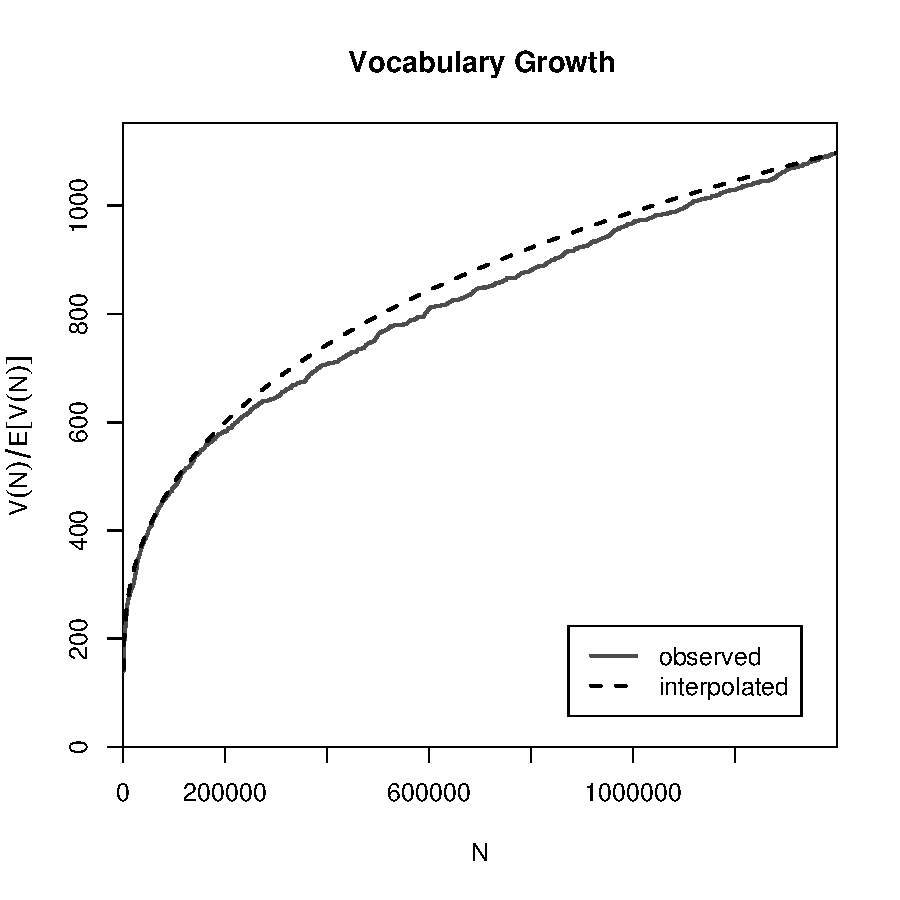
\includegraphics[width=6cm]{img/ri-vgc-binomial}
\end{center}

Interpolated curves look smoother, abstract away from fluctuations in
the original development profile, and they can be computed directly
from frequency spectra. However, if the relevant data are available,
it is a good idea to always take a look at the empirical curves as
well, as they might reveal the presence of strong non-randomness
patterns in the data, which invalidate the assumptions at the basis of
statistical model estimation. Indeed, the different shapes of the
empirical and expected curves for the \emph{ri-} data should be the
source of some mild concern about the validity of the assumptions even
in this case.

Similarly to spectrum objects, vgcs are also typed as regular R data
frames, so that their contents can be accessed with standard R data
frame syntax, when finer control over plotting and analysis parameters
is needed.

\subsection{Estimating V and other quantities at arbitrary sample
  sizes}

The vgc for \emph{ri-} shows that, had we sampled a smaller amount of
\emph{ri-} forms, our dataset would have contained a smaller number of
types. For example, according to the empirical vgc data, after the first
500,000 tokens, $V$ amounts to 761, vs.~1,098 for the whole dataset:%
\footnote{Note that this command only works because the vocabulary growth
  curve for \emph{ri-} happens to contain a data point for $N = 50000$ (=
  \texttt{5e+5}).}

\begin{verbatim}
> V(ItaRi.emp.vgc)[N(ItaRi.emp.vgc)==5e+5]
[1] 761
> V(ItaRi.spc)
[1] 1098
\end{verbatim}

The shape of the vgc also strongly suggests that, if we were to keep
sampling \emph{ri-} words, we would keep encountering new types, and
the vocabulary size would increase.  Thus, it is clear that the
vocabulary size $V$ is not a stable quantity, but that it increases as
sample size increases. Consequently, the $V$ in our sample cannot be
taken as a reliable estimate of the overall $V$ in the
\emph{population} we are sampling from (in our case, the population of
all possible \emph{ri-} prefixed verbs in Italian), nor of $V$s in
smaller and larger samples.

We already saw how binomial interpolation can be used to estimate $V$
for sample sizes smaller than $N$, the sample size at which the
frequency spectrum was computed. In order to \emph{extrapolate} $V$ to
larger samples (up to the whole population), we need to resort to
parametric statistical models for the distribution of frequencies in
the population (see \citealp{Evert:Baroni:2006b}; and see
\citealp[ch.~2]{Baayen:2001}, on why non-parametric extrapolation from
the observed frequency spectrum is problematic). The parametric models
appropriate for word frequency distributions (and distributions of
other linguistic types) belong to the family of
Large-Number-of-Rare-Events (LNRE) models. These are implemented in
zipfR as \textbf{LNRE model} objects. Currently, the toolkit supports
3 LNRE models: Generalized Inverse Gauss Poisson (\texttt{lnre.gigp};
\citealp[ch.~4]{Baayen:2001}), Zipf Mandelbrot (\texttt{lnre.zm};
\citealp{Evert:2004}) and finite Zipf Mandelbrot (\texttt{lnre.fzm};
\citealp{Evert:2004}). Mathematical details are provided in the
relevant references, whereas more information about the zipfR
implementations is available in the \texttt{lnre} and \texttt{lnre.*}
documentation entries. In future releases we might add support for the
other LNRE models introduced by \citet{Baayen:2001}, although the
tests of \citet{Evert:Baroni:2006a} suggest that the models currently
implemented in the package clearly outperform the others.

Coming back to our \emph{ri-} data, we will now use them to estimate a fZM
model. We call the \texttt{lnre} function with the string \texttt{"fzm"} and
the \emph{ri-} spectrum as arguments (the same syntax can be used with the
other models, substituting \texttt{"fzm"} with \texttt{"zm"} or
\texttt{"gigp"}, respectively).  The function automatically determines
suitable values for the 3 parameters of a fZM model by fitting the
\emph{expected} frequency spectrum of the model to the \emph{observed}
spectrum for \emph{ri-}.  Technically, this is achieved by non-linear
minimization of a cost function that quantifies the ``distance'' between
observed and expected spectrum, but you don't have to worry about such details
right now.  The command you need to enter is:

\begin{verbatim}
> ItaRi.fzm <- lnre("fzm", ItaRi.spc, exact=FALSE)
\end{verbatim}

We specified the name of the model we want to employ (here, fZM), the spectrum
to be used to estimate parameters and, by setting \texttt{exact} to FALSE, we
allowed approximations in the calculation of expected values (which improves
performance and numerical stability, but may lead to inaccurate results under
certain conditions; see the documentation of the \texttt{lnre} function for
details).  You might try now to re-estimate the model without the
\texttt{exact=FALSE} option (noting that the estimation procedure takes
considerably longer to complete).

As usual, \texttt{summary} provides you with a sketch of the object
you just created (you can also simply type the LNRE object name):

\begin{verbatim}
> summary(ItaRi.fzm)
finite Zipf-Mandelbrot LNRE model.
Parameters:
   Shape:          alpha = 0.3062077 
   Lower cutoff:       A = 4.224516e-23 
   Upper cutoff:       B = 0.1023475 
 [ Normalization:      C = 3.373107 ]
Population size: S = 78194057 
Sampling method: Poisson, approximations are allowed.

Parameters estimated from sample of size N = 1399898:
                V     V1     V2    V3    V4    V5    
   Observed: 1098 346.00 105.00 74.00 43.00 39.00 ...
   Expected: 1098 336.22 116.63 65.85 44.35 32.76 ...

Goodness-of-fit (multivariate chi-squared test):
         X2 df          p
   22.72643 13 0.04507887
\end{verbatim}

The \texttt{summary} function applied to a LNRE model returns the parameters
of the model and other useful information. In the case of a fZM model, this
includes the number of types in the population ($S$) and a comparison of
observed and expected values for the vocabulary size and the first five
spectrum elements.  Next, the \texttt{summary} reports the results of a
multivariate chi-squared test used to measure goodness of fit (see
\citealp[section 3.3]{Baayen:2001}). The lower the chi-squared statistic (and
the higher the p-value), the better the fit. Based on our experience (see,
e.g., \citealp{Evert:2004}), the goodness of fit reported in this case is
relatively good (although, in absolute terms, we would of course like to see
lower chi-squared values and higher p's). The fit to the observed spectrum can
also be visualized with a comparative spectrum plot. First, we produce the
spectrum of expected frequencies predicted by the fZM model at the sample size
we used to compute the model (i.e., the whole-dataset sample size):

\begin{verbatim}
> ItaRi.fzm.spc <- lnre.spc(ItaRi.fzm, N(ItaRi.fzm))
\end{verbatim}

Now, we plot the observed and expected spectra (the command reported
here produces a color plot; for the black and white version shown in
this tutorial you must, again, add the option \texttt{bw=TRUE} -- the
same is true for the plots below):

\begin{verbatim}
> plot(ItaRi.spc,ItaRi.fzm.spc,legend=c("observed","fZM"))
\end{verbatim}

\begin{center}
  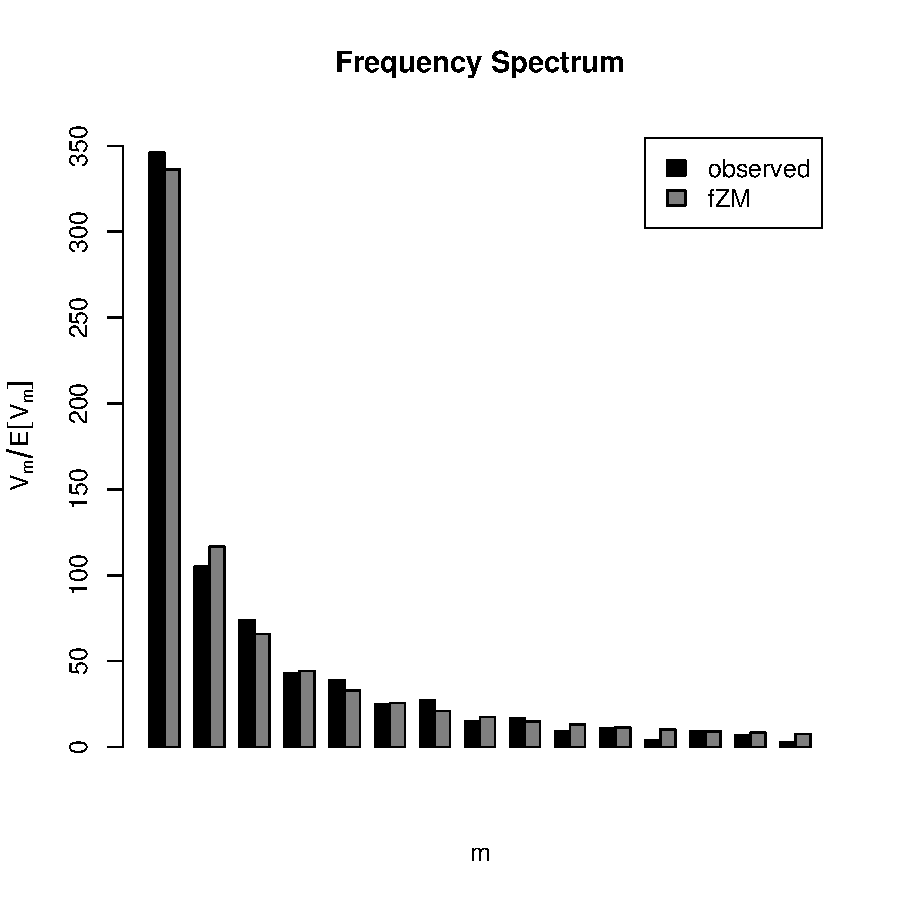
\includegraphics[width=6cm]{img/ri-spc-fzm}
\end{center}

The fZM model can now be used to obtain estimates of $V$ and $V_{m}$
(the spectrum elements) at arbitrary sample sizes. For example, we can
generate a vgc of expected $V$s up to a $N$ of 2.8 millions (about
twice the size of the \emph{ri-} sample) with the following command
(notice the syntax we use to request 100 equally spaced estimates of $V$
up to a sample size of 2.8 millions):

\begin{verbatim}
> ItaRi.fzm.vgc <- lnre.vgc(ItaRi.fzm, (1:100)*28e+3)
\end{verbatim}

It is worth mentioning that the function \texttt{lnre.vgc} can also provide
variance estimates for the vocabulary size (and the spectrum elements, when
relevant), via the \texttt{variances=TRUE} option. These could then be used to
plot confidence intervals around the growth curves. However, in our
experience, for many real-life datasets these intervals will be so narrow as
to be visually indiscernible from the curves (though not in the case of
\emph{ri-}).  We do not discuss these quantities here, but see the package
documentation (\texttt{lnre.vgc}, \texttt{plot.vgc}, etc.) and Baayen's book
\citep[ch.~3]{Baayen:2001}.

We now plot the expected curve together with the empirical one as
follows:

\begin{verbatim}
> plot(ItaRi.emp.vgc,ItaRi.fzm.vgc,N0=N(ItaRi.fzm),
+ legend=c("observed","fZM"))
\end{verbatim}

We obtain (a color version of) the following graph:

\begin{center}
  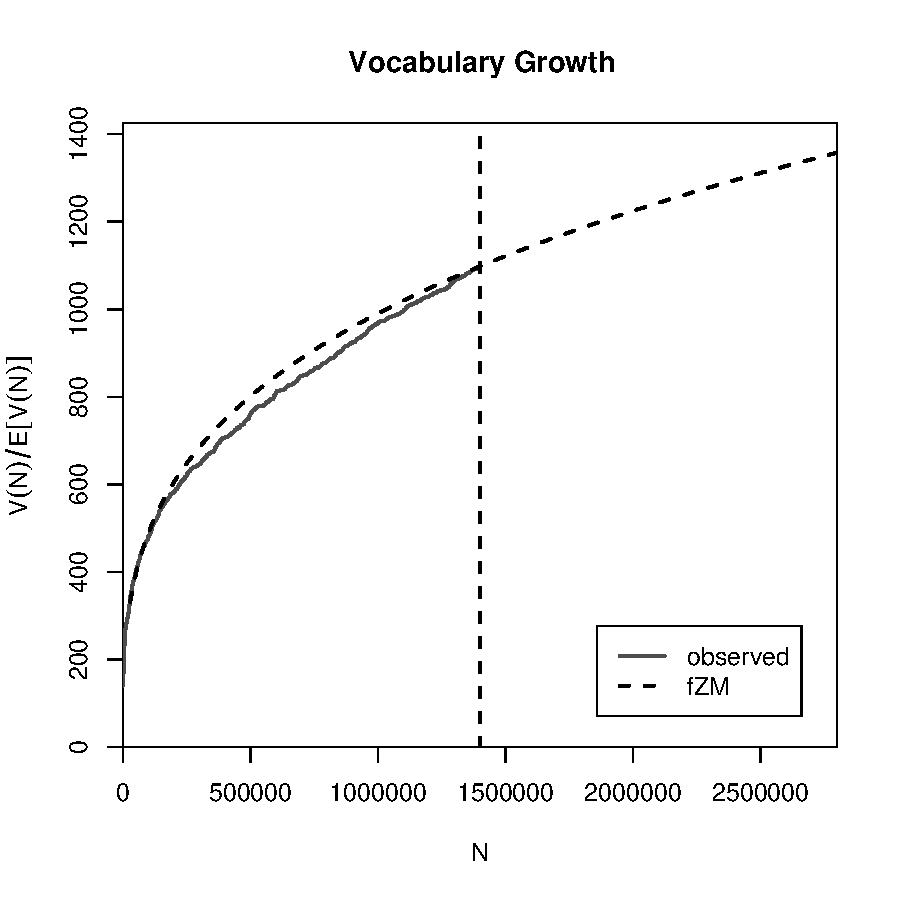
\includegraphics[width=6cm]{img/ri-vgc-fzm}
\end{center}

Notice the use of the argument \texttt{N0} to highlight the position
of $N_0$ (the estimation size) with a vertical line (see the
\texttt{plot.vgc} documentation).

As an exercise, you should now use the \emph{ri-} data to estimatea ZM and
GIGP models and look at the model summaries (it is instructive to compare the
predictions of the three models for the population vocabulary size $S$).  Then
add the expected values of the ZM and GIGP models to the comparative spectrum
and vgc plots for observed data vs.\ fZM.

Parameter estimation is one of the most difficult aspects of LNRE modeling.
We have made great efforts to implement a robust and efficient estimation
procedure for each LNRE model, so in most cases you can conveniently rely on
the default settings.  Sometimes parameter estimation will fail, however, or
produce an unsatisfactory fit to the observed frequency spectrum (as you will
be able to tell from the summary or comparative spectrum plot).  In these
cases, you can use three optional arguments of the \texttt{lnre} function to
fine-tune the estimation procedure.  The \texttt{cost} option allows you to
choose from a range of cost functions, while \texttt{m.max} determines how
many spectrum elements are included in the calculation of the selected cost
function.  The \texttt{method} option offers several different algorithms for
minimization of the cost function.  It can be interesting to look at
summaries, comparative spectrum plots and comparative vocabulary growth curves
of different LNRE models as well as the same model with different settings for
the parameter estimation procedure (and, of course, to test parameter
estimation for other data sets included in the \texttt{zipfR} package).  See
the \texttt{lnre} help page for detailed information about available options
and a long list of examples.  (Technical information for developers can be
found on the \texttt{lnre.details} and \texttt{estimate.model} help pages.)


\subsubsection{Evaluating extrapolation quality}

Although comparison with the empirical curve allows a visual assessment of the
goodness of fit of the \emph{interpolated} values (the expected $V$s up to the
observed sample size $N$), we have no way to visually assess the quality of
extrapolation beyond $N$, since we do not have observed values at sample sizes
larger than $N$. However, if we estimate the parameters of a LNRE model from a
subset of the data we have (i.e., using only $N_0$ tokens, where $N_0 < N$),
we can then compare extrapolation of this model up to our maximum observed
sample size $N$ to the empirical or interpolated growth curve up to $N$ (this
idea is explored in detail in \citealp{Evert:Baroni:2006a}).

If we have access to the original data, we can of course collect a
spectrum or type frequency list from the first $N_0$ tokens (outside
R), and import these data. However, here we will generate a spectrum
from a random subsample of the \texttt{ItaRi.spc} spectrum at
$N$. This allows us to illustrate another functionality of zipfR,
i.e., the possibility of building the frequency spectrum of a random
(sub)sample from an available frequency spectrum. In particular, with
the following function we create a subspectrum from a random sample of
$N_0=700,000$ tokens, about half the observed size:

\begin{verbatim}
> ItaRi.sub.spc <- sample.spc(ItaRi.spc, N=700000)
\end{verbatim}

The corresponding model:%
\footnote{If parameter estimation fails (as has been observed in one of our
  test runs), try omitting the \texttt{exact=FALSE} option, specify
  \texttt{method="NLM"}, or use a different cost function.}

\begin{verbatim}
> ItaRi.sub.fzm <- lnre("fzm", ItaRi.sub.spc, exact=FALSE)
> ItaRi.sub.fzm
finite Zipf-Mandelbrot LNRE model.
Parameters:
   Shape:          alpha = 0.2937111 
   Lower cutoff:       A = 1.824253e-21 
   Upper cutoff:       B = 0.08927604 
 [ Normalization:      C = 3.891048 ]
Population size: S = 16345389 
Sampling method: Poisson, approximations are allowed.

Parameters estimated from sample of size N = 700000:
               V     V1    V2    V3    V4   V5    
   Observed: 889 278.00 98.00 53.00 31.00 24.0 ...
   Expected: 889 261.11 92.21 52.45 35.48 26.3 ...

Goodness-of-fit (multivariate chi-squared test):
        X2 df          p
   25.8238 13 0.01795074
\end{verbatim}

Keep in mind that, because of the random subsampling process, your
subspectrum and, consequently, your LNRE model, will look different
from the ones presented here. In our case, the parameters of the model
are not too close to those we obtained when we used all the available
data to estimate it, and the estimated population size increased,
illustrating the undesirable dependency on sample size of LNRE model
estimation. Moreover, goodness of fit is lower than for the model
estimated from all the available data.

We generate a vgc up to the original $N$ from the
\texttt{ItaRi.sub.fzm} model:

\begin{verbatim}
> ItaRi.sub.fzm.vgc <- lnre.vgc(ItaRi.sub.fzm,
+ N=N(ItaRi.emp.vgc))
\end{verbatim}

Given that we took a random subsample, it is more appropriate to
compare the resulting vgc to one that is binomially interpolated from
$N$, rather than to the empirical vgc (we generated
\texttt{ItaRi.bin.vgc} in \ref{interpolation} above):

\begin{verbatim}
>  plot(ItaRi.bin.vgc, ItaRi.sub.fzm.vgc, N0=N(ItaRi.sub.fzm),
+ legend=c("interpolated","fZM"))
\end{verbatim}

This produces the following plot:

\begin{center}
  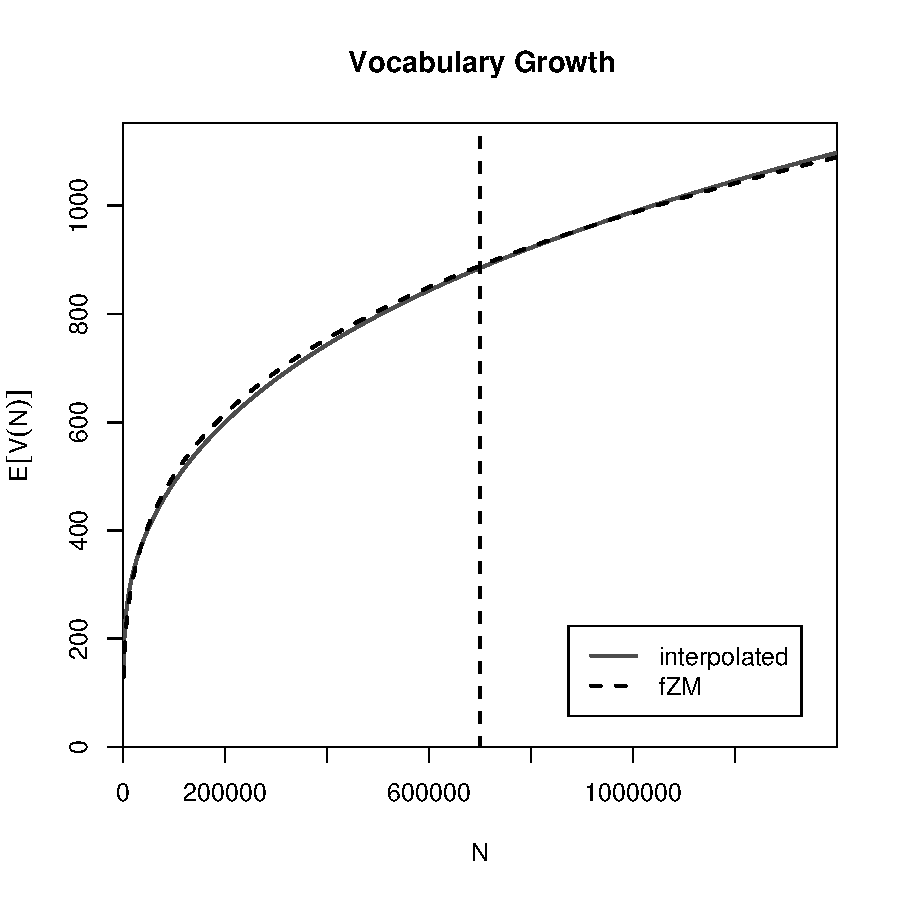
\includegraphics[width=6cm]{img/ri-vgc-fzm-extrapolation-quality}
\end{center}

The plot indicates that, despite the problems we mentioned above, the
fZM model provides a very reasonable match to the interpolated $V$
curve (it is hard to tell the two curves apart!)

Of course, the issue of evaluating the quality of LNRE models is more
complex than what we illustrated here. At the very least, one should
also look at models estimated from the first $N_0$ tokens, on top of
those obtained from a random subsample, and at averages of models
estimated from multiple random subsamples. The latter requires basic R
programming skills, to automatize the iterative estimation, vgc
generation and plotting procedure. We hope that future versions of the
zipfR toolkit will feature batch estimation and plotting functions, to
facilitate the process of running multiple randomization experiments.

\subsubsection{Comparing vocabulary growth curves of different
  categories}

For expository purposes, we focused here on the frequency distribution
of a single class (\emph{ri-} prefixed verbs in Italian). Of course,
it is typically more interesting to look at multiple frequency
distributions, e.g., by comparing their vgcs in order to determine
which of the classes under analysis is more productive. The zipfR
plotting functions make such comparisons easy, by accepting multiple
vgcs (or spc) data structures as input, and automatically determining
the best graphic parameters to plot them together.

As an example, we can compare the \emph{ri-} data with the data for
another Italian prefix, adjectival \emph{ultra-} (also extracted from
the \emph{la Repubblica} corpus with similar methods):

\begin{verbatim}
data(ItaUltra.spc)
\end{verbatim}

At first sight, one might think that \emph{ultra-} is less productive
than \emph{ri-}, given that its sample $V$ is half the one of
\emph{ri-}:

\begin{verbatim}
> V(ItaUltra.spc)
[1] 523
> V(ItaRi.spc)
[1] 1098
\end{verbatim}

However, the \emph{ultra-} sample is much smaller, making a direct
comparison meaningless:

\begin{verbatim}
> N(ItaUltra.spc)
[1] 3467
> N(ItaRi.spc)
[1] 1399898
\end{verbatim}

In order to compare the two word formation processes, we can compute a
LNRE model from the \emph{ultra-} data and then use it to extrapolate
the \emph{ultra-} growth curve up to the size of \emph{ri-}:

\begin{verbatim}
> ItaUltra.fzm <- lnre("fzm",ItaUltra.spc,exact=FALSE)
> ItaUltra.fzm
> ItaUltra.ext.vgc <- lnre.vgc(ItaUltra.fzm,N(ItaRi.emp.vgc))
> plot(ItaUltra.ext.vgc,ItaRi.bin.vgc,
+ legend=c("ultra-","ri-"))
\end{verbatim}


\begin{center}
  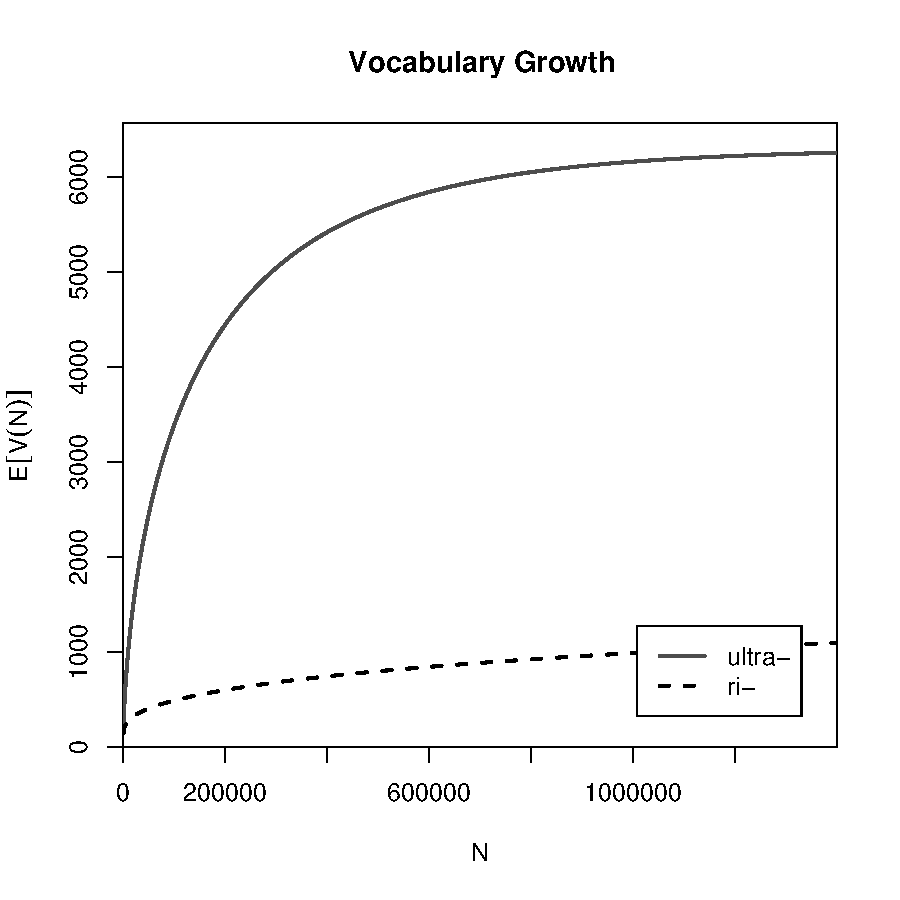
\includegraphics[width=6cm]{img/ultra-ri-vgc}
\end{center}

Interestingly, the extrapolation suggests that \emph{ultra-}, while
occurring more rarely, has the potential to generate many more words
than the already productive \emph{ri-} process.

You should now try to apply some of the functions illustrated here to
your own datasets (all you need is a frequency list or a frequency
spectrum for the process/class you are interested in), or to some of
the other example datasets that come with the zipfR package. You can
find out about the available datasets by typing:

\begin{verbatim}
> data(package="zipfR")
\end{verbatim}

You can obtain more information about a specific dataset by typing
its name preceded by the question mark, e.g.:

\begin{verbatim}
> ?ItaRi.spc
\end{verbatim}

As we mentioned at the beginning of this case study, while word
formation has been a classic area of application of word frequency
distribution modeling, techniques to estimate vocabulary size and
related quantities can find applications in any area of linguistics
where it makes sense to speak of a vocabulary of types, and the
overall size of this vocabulary is much larger than the size of the
observed vocabulary in our sample. For example, we could compare verbs
and adjectives (to assess whether verb formation is more productive
than adjective formation -- incidentally, you can try this with the
Brown corpus verb and adjective datasets available in the zipfR
package), or word pairs that occur in two different constructions (to
assess which construction is more productive), and so on and so
forth. With a bit of creativity in the definition of the target type
classes, vocabulary statistics modeling techniques can be applied to a
very wide range of linguistic problems.

\section{Case study 2: Estimating lexical coverage}

The first case study showed how to apply frequency distribution
analysis to a problem of (theoretical) linguistic interest, i.e.,
measuring the productivity/vocabulary size of a word formation
process. In this second case study we discuss a potential application
of the same tools to a practical problem in language engineering. This
case study is slightly more involved and it requires (just a little
bit) more R skills. If you feel that you've already learned enough
about zipfR to run your own experiments, feel free to skip to the last
section.

Many NLP algorithms heavily rely on specialized lexical
resources. Thus, performance on Out-Of-Vocabulary (OOV) types is lower
than when the input contains words/types that are stored in the
application lexicon. Among the language-related technologies that
crucially rely on a lexicon resource, we can mention part-of-speech
tagging and lexicalized probabilistic context-free grammars (see,
e.g., \citealp{Jurafsky:Martin:2000}).

It is therefore important to be able to estimate the proportion of OOV
words/types that we will encounter, given a lexicon of a certain size,
or, from a different angle, to determine how large our lexicon should
be in order to keep the OOV proportion below a certain threshold.

\subsection{Estimating the proportion of OOV types and tokens given a
  fixed size lexicon}

Consider the case in which we are developing an application that will
rely on a lexicon, and we are using the first 100k lemma tokens from
the Brown corpus \citep{Kucera:Francis:1967} as our development
resource. The frequency spectrum of this subset of the Brown is part
of the zipfR datasets and, if the zipfR library is loaded, it can be
imported as follows:

\begin{verbatim}
> data(Brown100k.spc)
\end{verbatim}

The vocabulary size of this set is:

\begin{verbatim}
> V(Brown100k.spc)
[1] 12780
\end{verbatim}

We decide that we can afford to write lexical entries of the kind
required by our application for all the lemmas that occur at least two
times in our dataset, i.e., our lexicon of seen types will have the
following size (obtained by subtracting the hapax type count from the
overall vocabulary size):

\begin{verbatim}
> Vseen <- V(Brown100k.spc) - Vm(Brown100k.spc,1)
> Vseen
[1] 6477
\end{verbatim}

In this way, we will cover about 50\% of the \emph{types} in our
development set, whereas the other 50\% will count as OOV types:

\begin{verbatim}
> Vseen / V(Brown100k.spc)
[1] 0.5028276
\end{verbatim}

However, given that the OOV lemmas are hapax legomena, they actually
account for a much lower proportion of the overall \emph{tokens}:

\begin{verbatim}
>  Vm(Brown100k.spc,1) / N(Brown100k.spc)
[1] 0.06303
\end{verbatim}

I.e., given our choice to insert in the lexicon all lemmas that occur
at least twice in the development set, we cover about 94\% of the
tokens in the development set itself, while the remaining 6\% of the
tokens belong to OOV types.

However, what will happen when we use our application on a larger
input? What proportion of OOV types and tokens should we expect? To
answer this question, we estimate a LNRE model from the available
spectrum, we extrapolate to larger $N$s via the model, and we check
what proportion of the types and tokens will be maximally covered by
our $V_{seen}$ entries at these larger $N$s. Of course, we have to
make the very delicate assumption that the input that our application
will see is very similar to the 100k Brown fragment we used as our
development set; i.e., that larger texts fed to the application are
larger random samples of the population we sampled our development set
from (indeed, here we also assume that the development fragment itself
is always part of the larger input). The assumption might be
reasonable if, e.g., our application is targeted at automatically
annotating the remaining 900k tokens from the Brown, and for some
reason we do not have access to them during development (this sounds
silly in the case of the Brown, but it might be a realistic scenario
when the corpus we are working on is still in the construction phase);
or if the application will be used to parse a certain specialized
language, and the development set is made of texts from that language.

In this case study, we estimate a ZM model from our data:

\begin{verbatim}
> Brown100k.zm <- lnre("zm", Brown100k.spc)
> Brown100k.zm
Zipf-Mandelbrot LNRE model.
Parameters:
   Shape:          alpha = 0.6438654 
   Upper cutoff:       B = 0.007900669 
 [ Normalization:      C = 1.996773 ]
Population size: S = Inf 
Sampling method: Poisson, with exact calculations.

Parameters estimated from sample of size N = 100000:
                 V      V1      V2      V3     V4     V5    
   Observed: 12780 6303.00 2041.00 1067.00 648.00 472.00 ...
   Expected: 12780 8273.68 1473.27  665.98 392.29 263.31 ...

Goodness-of-fit (multivariate chi-squared test):
         X2 df p
   4953.447 14 0
\end{verbatim}

Notice that $S$ (population vocabulary size) is infinite, since the ZM
model, unlike fZM, does not assume a finite population. Notice also
that the multivariate chi-squared test suggests a very poor fit. This
seems to be a general property of ZM \citep{Evert:2004} and one that,
interestingly, does not always imply poor extrapolation quality
\citep{Evert:Baroni:2006a}.

We can use the model we just estimated to generate expected $V$s at
arbitrary $N$s, in order to calculate the proportion of OOV types we
are likely to encounter. For example, we can see what will this
proportion be if the input contains 1, 10, 100 million tokens (notice
the function \texttt{EV} that, given a model, produces the expected $V$
values for a vector of $N$s):

\begin{verbatim}
> EV(Brown100k.zm, c(1e6, 10e6,100e6))
[1]   56523.8  249179.5 1097670.7
\end{verbatim}

Thus, the proportions of in-lexicon types for inputs of 1, 10, 100
million tokens (assuming that our development set is a subset of the
input, so that all the types in our lexicon are used) are:

\begin{verbatim}
> Vseen / EV(Brown100k.zm, c(1e6,10e6,100e6))
[1] 0.114588909 0.025993308 0.005900677
\end{verbatim}

Equivalently, the proportions of OOV types are:

\begin{verbatim}
>  1 - (Vseen / EV(Brown100k.zm, c(1e6,10e6,100e6)))
[1] 0.8854111 0.9740067 0.9940993
\end{verbatim}

We can get a sense of how good the estimates are by importing the
spectrum for the whole Brown, and comparing the number of types in the
whole corpus to the number of expected types at the same sample size
according to the model. Importing the spectrum:

\begin{verbatim}
data(Brown.spc)
\end{verbatim}

Observed $N$ and $V$:

\begin{verbatim}
>  N(Brown.spc)
[1] 1006770
>  V(Brown.spc)
[1] 45215
\end{verbatim}

The model-based estimate of $V$ at the same $N$:

\begin{verbatim}
> EV(Brown100k.zm,N(Brown.spc)) 
[1] 56770.19
\end{verbatim}

This is relatively close to the observed value (although it overestimates the
true vocabulary growth), and consequently the empirical and estimated OOV
ratios are reasonably close:

\begin{verbatim}
> 1 - (Vseen / V(Brown.spc))
[1] 0.856751
> 1 - (Vseen / EV(Brown100k.zm, N(Brown.spc)))
[1] 0.8859084
\end{verbatim}

On to the probably more interesting question of estimating the
proportion of OOV \emph{tokens} in larger samples, given our lexicon
of 5,157 types. First, we generate a model-derived spectrum at the
desired $N$. From this, we obtain the expected $V$ estimate and, by
subtracting $V_{seen}$ from $V$, an estimate of the number of OOV
types ($V_{OOV}$). At this point, we make the best case scenario (but
not completely unreasonable) assumption that the OOV types will always
be less frequent than the types that are already in our lexicon. Thus,
we first look at the number of hapax legomena in the estimated
spectrum. If this value is below $V_{OOV}$, we also add the number of
types occurring twice, three times, etc., until we reach a value close
to $V_{OOV}$. Once we determined (roughly) up to what frequency class
the OOV types extend, we can calculate their overall token frequency
by multiplying the number of types in each of the OOV classes by the
corresponding frequency and summing up (to get the number of hapax
legomenon tokens, we multiply the number of hapax types by 1, to get
the number of tokens of types that occur twice, we multiply the number
of twice-occurring types by 2, and so on -- finally, to get the
overall token frequency of the classes involved, we sum all these
values).

We estimate the spectrum from our ZM model at $N=1,170,811$, so that
the result will be directly comparable to the observed spectrum from
the whole Brown:

\begin{verbatim}
> Brown.zm.spc <- lnre.spc(Brown100k.zm, N(Brown.spc))
\end{verbatim}

By default, \texttt{lnre.spc} generates the first 100 spectrum
elements (ideally, we would like to generate a full frequency
spectrum: however, certain LNRE models -- in particular GIGP -- incur
into numerical problems with higher spectrum elements; hence the
conservative default). The estimate of $V_{OOV}$ (notice that we
cannot extract the expected $V$ from the estimated spectrum, since the
latter does not contain all frequency classes):

\begin{verbatim}
> EV(Brown100k.zm, N(Brown.spc)) - Vseen 
[1] 50293.19
\end{verbatim}

Starting from the lowest expected frequency class, let us sum types
until we reach a value close to 50,293:

\begin{verbatim}
> sum(Vm(Brown.zm.spc, 1))
[1] 36597.44
> sum(Vm(Brown.zm.spc, 1:2))
[1] 43114.25
...
> sum(Vm(Brown.zm.spc, 1:6))
[1] 49805.72
\end{verbatim}

Given that we are working with rough estimates anyway, we take the sum
of the types in the lowest 6 frequency classes to be close enough to
the estimated $V_{OOV}$. Thus, to calculate the number of OOV tokens
we multiply the types in each of these classes by the corresponding
frequencies and sum:

\begin{verbatim}
> Noov.zm <- sum(Vm(Brown.zm.spc, 1:6) * c(1:6))
> Noov.zm
[1] 76307.01
\end{verbatim}

In proportion:

\begin{verbatim}
> Noov.zm / N(Brown.spc)
[1] 0.07579389

\end{verbatim}

I.e., about 7.5\% of the overall tokens belong to OOV types. Let us
compare this to the same quantity computed from the full observed
frequency dataset (the spectrum of frequencies in the whole
Brown). $V_{OOV}$ from the observed data:

\begin{verbatim}
> V(Brown.spc) - Vseen
[1] 38738
\end{verbatim}

Approximating this value from the low end of the spectrum:

\begin{verbatim}
> sum(Vm(Brown.spc, 1))
[1] 19130
> sum(Vm(Brown.spc, 1:2))
[1] 25588
...
>  sum(Vm(Brown.spc, 1:13))
[1] 38756
\end{verbatim}

Thus, the $N_{OOV}$ estimate from the observed frequency spectrum is:

\begin{verbatim}
> Noov.emp <- sum(Vm(Brown.spc, 1:13) * c(1:13))
> Noov.emp
[1] 108120
> Noov.emp / N(Brown.spc)
[1] 0.1073929
\end{verbatim}

The model-derived estimate of the proportion of OOV tokens is
considerably lower than the one derived from the observed spectrum (in
accordance with the general tendency of LNRE models to underestimate
type-related quantities in extrapolation -- see
\citealp{Evert:Baroni:2006a}); however, the model-based proportion
still seems reasonable as a ballpark estimate.


\subsection{Determining lexicon size}

Suppose that, in a certain project, we will have to develop a lexical
resource, and we are in the phase in which we need to decide how large
it should be. One approach to this task is to estimate how many types
we should enter in the lexicon to achieve a certain coverage on input
of various sizes, and use this estimate as a guide in deciding the
size of the target lexicon.

For example, suppose that we want to try to reach 95\% coverage, i.e.,
no more than about 5\% OOV tokens, given an expected input of 10
million words. With our usual ZM model, we estimate the spectrum at
$N=10$ millions:

\begin{verbatim}
> Brown10M.zm.spc <- lnre.spc(Brown100k.zm, 10e6)
\end{verbatim}


5\% of 10 millions is 500,000, thus we must sum up the lowest
frequency spectrum elements multiplied by the corresponding
frequencies until we reach a value close to 500,000. By trial and
error, we find that we can get a reasonably close value by summing up
the token frequencies of the first 18 frequency classes (trial and
error can be made less typing-intensive by using the R function
\texttt{cumsum} instead of \texttt{sum}, in order to obtain a vector
of cumulative sums):

\begin{verbatim}
> sum(Vm(Brown10M.zm.spc, 1:18) * c(1:18))
[1] 501239.5
\end{verbatim}

This corresponds to a $V_{OOV}$ of:

\begin{verbatim}
> sum(Vm(Brown10M.zm.spc, 1:18))
[1] 233847
\end{verbatim}

Thus, the number of types we should insert in our lexicon to have
hopes to cover 95\% of the tokens in a 10 million token input is:

\begin{verbatim}
> EV(Brown100k.zm, 10e6) - sum(Vm(Brown10M.zm.spc, 1:18))
[1] 15332.51
\end{verbatim}

Now, as an exercise, find out how many types we need in the lexicon in
order to cover 95\% of the tokens in a 100 million token input.  Is
this quantity much higher than the one needed for the 10 million token
input?  Notice that you will need to use the \texttt{m.max} argument of
\texttt{lnre.spc} in order to obtain more than 100 spectrum elements.


\section{Directions for further exploration}

The case studies in this tutorial illustrate many functionalities of
the zipfR package. You can find out more about the package by
exploring its documentation.

To practice, you can repeat the procedures above experimenting with
different LNRE models and exploring other zipfR datasets. Of course,
it is probably more interesting for you to work with your own data. As
long as you can convert them to a plain frequency list format, you
will be able to import them into zipfR using \texttt{read.tfl}. On the
zipfR website (\url{http://purl.org/stefan.evert/zipfR}) you can also
find a script to compute empirical vocabulary growth curves from plain
tokenized corpus data.

Finally, we would like to remind you that zipfR, like R, is an open source,
GPL-licensed project. We invite you to contribute to its further development
with bug reports, encouragement, suggestions, and code!




\begin{thebibliography}{}

\bibitem[Baayen, 1992]{Baayen:1992} Harald Baayen (1992). Quantitative
  aspects of morphological productivity. {\em Yearbook of Morphology
    1991}, 109-150.
  
\bibitem[Baayen, 2001]{Baayen:2001} Harald Baayen (2001). \emph{Word frequency
    distributions}. Dordrecht: Kluwer.

\bibitem[Baroni et al., 2004]{Baroni:etal:2004} Marco Baroni, Silvia
  Bernardini, Federica Comastri, Lorenzo Piccioni, Alessandra Volpi,
  Guy Aston and Marco Mazzoleni (2004). Introducing the ``la
  Repubblica'' corpus: A large, annotated, TEI(XML)-compliant corpus
  of newspaper Italian. \emph{Proceedings of LREC 2004}, 771-1774.
  
\bibitem[Dalgaard, 2002]{Dalgaard:2002} Peter Dalgaard (2002).
  \emph{Introductory statistics with R}. New York: Springer.

\bibitem[Evert, 2004]{Evert:2004} Stefan Evert (2004). A simple LNRE
  model for random character sequences. \emph{Proceedings of JADT
    2004}, 411-422.
 
\bibitem[Evert and Baroni, 2006a]{Evert:Baroni:2006a} Stefan Evert and
  Marco Baroni (2006a). Testing the extrapolation quality of word
  frequency models. \emph{Proceedings of Corpus Linguistics 2005}.

\bibitem[Evert and Baroni, 2006b]{Evert:Baroni:2006b} Stefan Evert and
  Marco Baroni (2006b). ZipfR: Working with words and other rare
  events in R. \emph{R User Conference 2006}.

\bibitem[Jurafsky and Martin, 2000]{Jurafsky:Martin:2000} Daniel
  Jurafsky and James Martin. 2000. \emph{Speech and language
    processing}. Upper Saddle River: Prentice Hall.

\bibitem[Ku\v{c}era and Francis, 1967]{Kucera:Francis:1967} Henry
  Ku\v{c}era and Nelson Francis (1967). {\em Computational analysis of
    present-day American English}. Providence: Brown University Press.

% \bibitem{Manning:Schuetze:1999} Christian Manning and Hinrich Sch�tze
%   (1999). \emph{Foundations of statistical natural language
%     processing}. Cambridge (Mass.): The MIT Press.

\end{thebibliography}

\end{document}
